\documentclass[a4paper,11pt,fleqn]{scrartcl}%fleqn pour aligner les equations à gauche

\usepackage{../../Styles/Eval}

\newcommand{\chnum}{Chapitre 12}
\newcommand{\chtitle}{Mouvements dans un champ uniforme}
\newcommand{\dtype}{Eval}

\begin{document}
	\maketitle
\section*{Le scanner à rayons X}
La radiographie réalisée par un scanner à rayons X est une technique d'imagerie médicale utile dans le diagnostique de nombreuses pathologies.\\
Le scanner crée un saisceau à rayons X à l'aide d'un tube à rayons X ou de Coolidge.
\begin{figure}[h!]
    \centering
    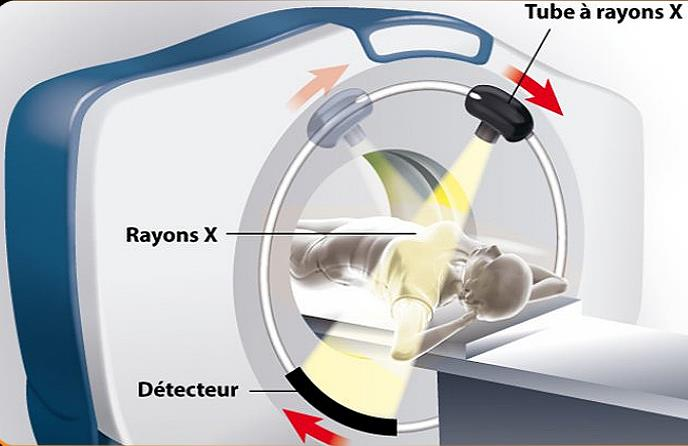
\includegraphics[width = .5\linewidth]{Ressources/TSPE_DS2_25_Fig5.png}
\end{figure}
Dans ce tube à rayons X, une tension élevée $U$ est maintenue entre un filament cathodique. borne négative, et une anode tournante, norne positive (doc.~\ref{doc5} et~\ref{doc6}). Un courant électrique provoque l'échauffement d'un filament situé à la cathode. L'agitation des électrons présents augente et une partie d'entre eux est éjectée du filament au point $O$, avec une vitesse négligeable. La tension $U$ accélère les électrons du point $O$ vers l'anode en tungstène. Denevus très énergétiques, ils frappent l'anode, ce qui produit des rayons X. Pour obtenir ces rayons X, chaque électron doit avoir acquis une énergie cinétique égale à \SI{6,4E-15}{J} au minimum.

\begin{figure}[h!]
    \begin{minipage}{.49\linewidth}
       \caption{Schéma du tube à rayons X}
       \label{doc5}
       \centering
       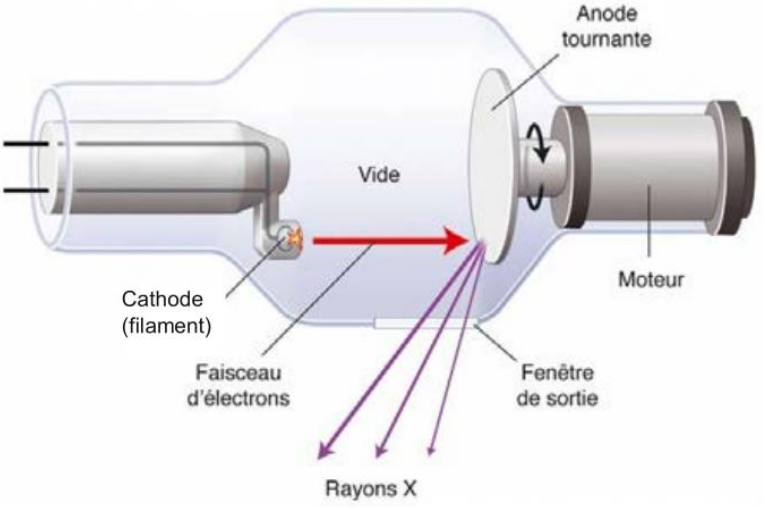
\includegraphics[width=.8\linewidth]{Ressources/TSPE_DS2_25_Fig6.png} 
    \end{minipage}
    \begin{minipage}{.49\linewidth}
       \caption{Schéma simplifié}
       \label{doc6}
       \centering
       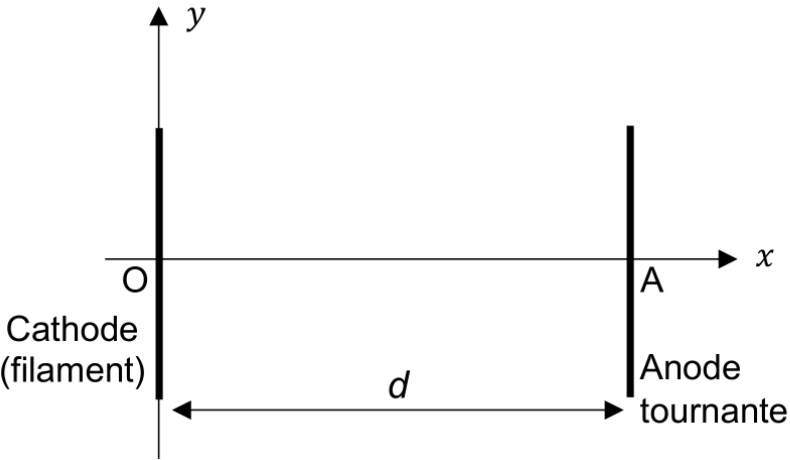
\includegraphics[width=.8\linewidth]{Ressources/TSPE_DS2_25_Fig7.png} 
    \end{minipage}
\end{figure}

Le but de cet exercice est de calculer la tension à appliquer entre la cathode et l'anode pour que le faisceau d'électrons parvienne à provoquer l'émission de photons X au niveau de l'anode. On considèrera l'électrons comme système d'étude assimilé à un point matériel dont on négligera le poids. Son mouvement sera étudié dans le référentiel terrestre considéré comme galiléen. on mouvement sera étudié dans un référentiel terrestre considéré comme galiléen. À l'instant initial, l'électron est situé au point $O$ et sa vitesse est considérée comme nulle.\\

\begin{data}
    \begin{itemize}
        \item Masse de l'électron : $m = \SI{9,1E31}{kg}$
        \item Charge de l'électrons : $q = -e = \SI{-1,6E-19}{C}$
    \end{itemize}
\end{data}

\begin{enumerate}
    \item Reproduire le doc.~\ref{doc5} puis tracer, entre la cathode et l'anode, sans préciser d'échelle :\begin{itemize}
        \item le vecteur champ électrique supposé uniforme $\vv{E}$
        \item la force $\vv{F}$ que subit un électron situé en un point de l'axe ($0x$)
    \end{itemize}
    \item Donner l'expression vectorielle de $\vv{F}$ en fonction de $e$ et $\vv{E}$.
    \item Montrer que les coordonnées du vecteur accélération $\vv{a}$ de l'électron, exprimées dans le repère ($Oxy$) du doc.~\ref{doc5}, sont $a_x = \dfrac{e\cdot U}{m \cdot d}$ et $a_y = 0$.
    \item En déduire le coordonnées du vecteur vitesse de l'électron selon l'axe ($Ox$), notée $v_x$. Établir que $x$ d'écrit $ \dfrac{1}{2} \cdot \left(\dfrac{e\cdot U}{m \cdot d}\right) \cdot t^2$.
    \item Donner l'expression litterale de $T_A$, l'instant où l'électron atteint l'anode (au point $A$) située à la distance $d$ de $O$
    \item Grâce aux deux questions précédentes, en déduire que l'expression de la vitesse de l'électron au niveau de l'anode est $v_A = \sqrt{\dfrac{2\cdot e \cdot U}{m}}$.
    \item Répondre à la problématique de l’exercice "trouver la tension minimale à appliquer entre la cathode et l’anode pour que le faisceau d’électron parvienne à provoquer l’émission de photons X an niveau de l’anode".
\end{enumerate}

\end{document}
